\documentclass[border=10pt]{standalone}
\usepackage{tikz}
\usetikzlibrary{calc}
\usetikzlibrary{arrows,positioning,shapes.geometric}
% for i in 1 2 3; do pdftoppm -png process_video$i.pdf > process_video$i.png; done

\begin{document}
    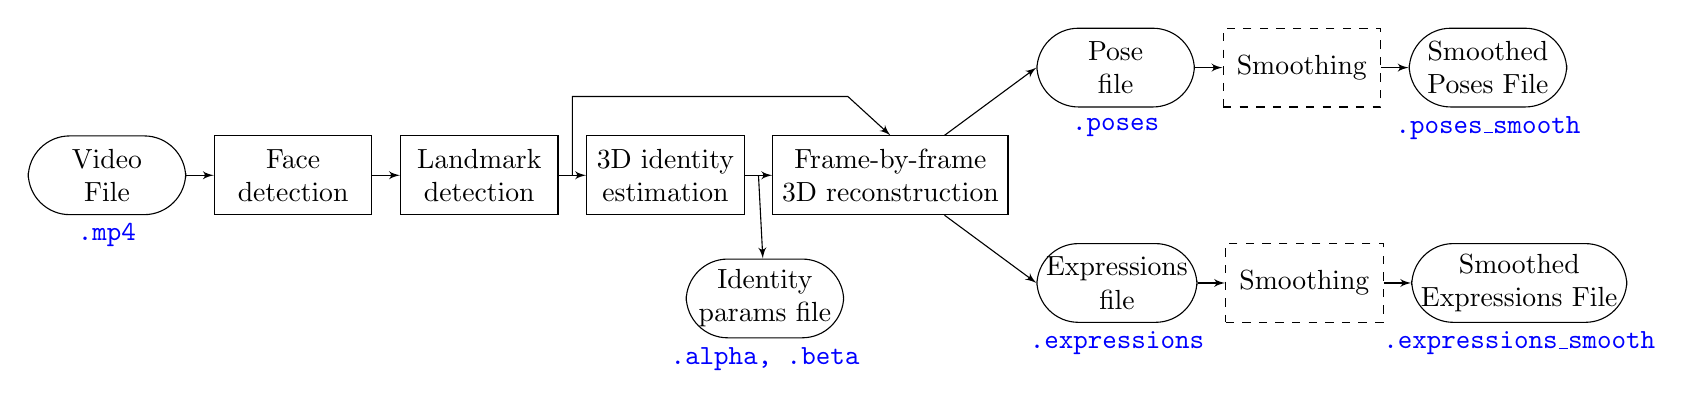
\begin{tikzpicture}[>=latex']
        \tikzset{block/.style= {draw, rectangle, align=center,minimum width=2cm,minimum height=1cm}, 
        dblock/.style= {draw=black,dashed,  align=center,minimum width=2cm,minimum height=1cm},
        int/.style={minimum size=2em,font=\ttfamily,text=blue},
        rblock/.style={draw, shape=rectangle,rounded corners=1.5em,align=center,minimum width=2cm,minimum height=1cm},
        input/.style={ % requires library shapes.geometric
        draw,
        trapezium,
        trapezium left angle=60,
        trapezium right angle=120,
        minimum width=2cm,
        align=center,
        minimum height=1cm
    },
        }
        \node [rblock]  (input) {Video\\File};
        \node [block, right =0.35cm of input] (face_detect) {Face\\detection};
        \node [block, right =0.35of face_detect] (lmk_detect) {Landmark\\detection};
        \node [block, right =0.35cm of lmk_detect] (identity) {3D identity\\estimation};
        \node [block, right =0.35cm of identity] (rec) {Frame-by-frame\\3D reconstruction};
        \node [rblock, below right =0.55cm and -0.75cm of identity] (id_file) {Identity\\params file};
        \node [rblock, above right =0.5cm of rec] (pose) {Pose\\ file};
        \node [rblock, below right =0.5cm of rec] (exp) {Expressions\\ file};
        %\node [rblock, below right =0.8cm and 0.5cm of rec] (lmks) {2D landmarks\\ file};
        \node [int, below=-0.1cm of input] (inp_ext) {.mp4};
        \node [int, below=-0.1cm of id_file] (id_ext) {.alpha, .beta};
        \node [int, below=-0.1cm of pose] (pose_ext) {.poses};
        \node [int, below=-0.1cm of exp] (exp_ext) {.expressions};

        \node [dblock, right=0.35cm of pose] (pose_sm_proc) {Smoothing};
        \node [dblock, right=0.35cm of exp] (exp_sm_proc) {Smoothing};
        
        \node [rblock, right =0.35cm of exp_sm_proc] (exp_sm) {Smoothed\\ Expressions File};
        \node [rblock, right =0.35cm of pose_sm_proc] (pose_sm) {Smoothed\\ Poses File};
        \node [int, below=-0.1cm of exp_sm] (exp_sm_ext) {.expressions\_smooth};
        \node [int, below=-0.1cm of pose_sm] (pose_sm_ext) {.poses\_smooth};
%        \node [int, below=-0.1cm of lmks] (lmk_ext) {.2Dlandmarks};

%% paths
        \path[draw,->] (input) edge (face_detect)
                    (face_detect) edge (lmk_detect)
                    (lmk_detect) edge (identity)
                    (identity) edge (rec)
                    (rec) edge (pose.west)
                    (rec) edge (exp.west)
%                    (rec) edge (lmks.west)
                    ($(identity.east)!.5!(rec.west)$) edge  (id_file)
                    ($(lmk_detect)!.5!(identity)$) -- ++(0,1cm) -- ++(3.5cm,0) -- (rec.north)
                    (pose) edge (pose_sm_proc)
                    (pose_sm_proc) edge (pose_sm)
                    (exp) edge (exp_sm_proc)
                    (exp_sm_proc) edge (exp_sm)
                    ;
    \end{tikzpicture}
    
\end{document}